\section{Transformada de Fourier}

En matemáticas se llama transformada al mecanismo que convierte un problema de un tipo a otro, este último presumiblemente más fácil de resolver. El modo de hacerlo es resolver primero el problema transformado, para después transformar de regreso y así obtener la solución del problema original. En el caso de la transformada de Fourier (o transformada de Lapace como se verá más adelante) los problemas con valores iniciales son convertidos en problemas algebraicos, un proceso que se puede ilustrar del modo siguiente
\begin{figure}[ht]
  \centering
  \begin{tikzpicture}[node distance=5mm,
    terminal/.style={
      % The shape:
      rectangle,minimum size=6mm,rounded corners=3mm,
      % The rest
      very thick,draw=black!50,
      top color=white,bottom color=black!20,
      font=\ttfamily
    }]
    \node (start) [terminal] {problema con valores iniciales};
    \node (algebraic) [terminal,below=of start] {problema algebraico};
    \node (solution_alg) [terminal,below=of algebraic] {solución del problema algebraico};
    \node (end) [terminal,below=of solution_alg] {solución del problema con valores iniciales};

    \path (start) edge[->] (algebraic) 
    (algebraic) edge[->] (solution_alg)
    (solution_alg) edge[->] (end);
  \end{tikzpicture}
\end{figure}

Veremos también que la transformada de Fourier es una herramienta básica en el análisis de señales aperiódicas que tienen energía finita. En este sentido, la transformada de Fourier juega el mismo papel que las series de Fourier para señales periódicas.

Antes de pasar a ver la definición de transformada de Fourier, vamos a definir el vocabulario que se utilizará para evitar ambigüedades.
\begin{definition}
  Llamamos frecuencia no angular de una función $f(t)$ a 
  $$
  f=\frac{1}{T}
  $$
  Que implícitamente define lo que llamamos período de $f(t)$:
  $$
  T=\frac{1}{f}
  $$

  Por otro lado, llamamos frecuencia angular (o solo frecuencia) al valor:
  $$
  \omega =2\pi \cdot f = \frac{2\pi}{T}
  $$
  Este valor es el que utilizaremos en su mayoría. En caso de precisar el valor de $f$, diremos \textit{frecuencia no angular}.
  \label{def:frecuencia}
\end{definition} 

\subsection{Definición}

Antes de dar la definición rigurosa de transformada de Fourier, vamos a motivar dicha definición a partir de las series de Fourier. Sea $f:\mathbb{R}\to\mathbb{C}$ una función que, en principio, consideraremos restringida a un intervalo finito de tiempo $T$. Podemos expresar $f(t)$ mediante su serie exponencial de Fourier:
\begin{equation}
    f(t)=\sum_{k=-\infty}^{\infty} C_k e^{j k \omega t}
\end{equation}
donde $\omega = \frac{2\pi}{T}$ es la frecuencia fundamental y los coeficientes vienen dados por:
\begin{equation}
    C_k = \frac{1}{T}\int_{-T/2}^{T/2}f(t) e^{-jk\omega t} dt
    \label{eq:coeficientes_serie}
\end{equation}
Aquí, $f(t)$ es periódica con periodo $T$. Un detalle que no debe pasar por alto es que la función dada, $f(t)$, ya cuenta con sus propias características, esté o no representada por una serie. Si suponemos a esta presunta $f(t)$ periódica, entonces, ella tendrá su período $T$ y, por lo tanto, su frecuencia $\omega$. Por ejemplo $f(t)=\cos(t)$ tiene por sí misma $T=2\pi$ y $\omega=1$. Al representar una determinada $f(t)$ mediante una serie de Fourier, se está escribiendo esta misma función como una combinación lineal de senos y cosenos. 

Una representación gráfica hipotética de la amplitud de las frecuencias componentes de $f(t)$ podría ser la gráfica que se muestra en la figura \ref{fig:grafico_de_frecuencia}.
\begin{figure}[ht]
  \centering
  \begin{tikzpicture}
    \draw[->,gray] (-4.8,0) -- (4.8,0) node[right] {$k\omega$};
    \draw[->,gray] (0,-.1) -- (0,2.8) node[above] {$|C_k|$};

    \draw[red,very thick,fill] (0,0) node[below] {\color{black}\scriptsize$0$} -- (0,2) circle (2pt) node[above=3pt,fill=white,inner sep=0pt] {\scriptsize$C_0$};
    \foreach \k\i in {1/2,2/3,3/4,4/5} {
      \draw[red,very thick,fill] (\k,0) node[below] {\color{black}\scriptsize$\k\omega$} -- ($(\k,1/\i*2)$) circle (2pt) node[above] {\scriptsize$\lvert C_\k\rvert$};
      \draw[red,very thick,fill] (-\k,0) node[below] {\color{black}\scriptsize$-\k\omega$} -- ($(-\k,1/\i*2)$) circle (2pt) node[above] {\scriptsize$\lvert C_\k\rvert$};
    }
    \draw[dashed, smooth] plot coordinates {
      (-4,0.4) (-3,0.5) (-2,0.6666) (-1,1) (0,2)
      (1,1) (2,0.6666) (3,0.5) (4,0.4)
    };
  \end{tikzpicture}
  \caption{Representación de la amplitud de frecuencia discreta o de línea.}
  \label{fig:grafico_de_frecuencia}
\end{figure}
Esto nos sirve para definir algunos conceptos.
\begin{definition}[Curva envolvente]
  Llamamos envolvente a la curva suave que une cada punto $C_k$ en la gráfica de amplitud de frecuencias.
\end{definition}
\begin{definition}[Densidad espectral]
  Llamamos densidad espectral de frecuencia a la cantidad que nos dice que tan concentrada está la amplitud ($C_k$) alrededor de la frecuencia $\omega_k$.
\end{definition}
Ahora, nuestro objetivo es analizar funciones \textbf{no periódicas} (o aperiódicas). Una función aperiódica puede interpretarse matemáticamente como una función periódica cuyo periodo tiende a infinito ($T \to \infty$).

Si observamos la ecuación \ref{eq:coeficientes_serie}, vemos que $C_k$ representa la amplitud de la frecuencia discreta $k\omega$. A medida que aumentamos el periodo $T$:
\begin{itemize}
    \item La frecuencia fundamental $\omega = 2\pi/T$ disminuye, haciéndose cada vez más pequeña. 
    \item Los armónicos en el gráfico de frecuencias se juntan cada vez más. Veamos este último inciso más en detalle con un breve ejemplo.
\end{itemize}
\begin{example}
  Si miramos la figura \ref{fig:grafico_de_frecuencia}, vemos que $f(t)$, con su periodo original $T$ tiene una frecuencia determinada $\omega$. Si aumentamos el periodo tal que $T'=2T$, entonces la nueva frecuencia $\omega'=2\pi/(2T)=\omega/2$. Es decir, esta nueva $g(t)$ que es idéntica a $f(t)$ pero tiene un período dos veces mayor, tiene la mitad de frecuencia. Esto conlleva a que su gráfico de frecuencias comparado con el de $f(t)$ sea como muestra la figura \ref{fig:grafico_de_frecuencia_de_g}
  \begin{figure}[ht]
    \centering
    \begin{tikzpicture}
      \draw[->,gray] (-4.8,0) -- (4.8,0) node[right] {$k\omega$};
      \draw[->,gray] (0,-.1) -- (0,1.8) node[above] {$|C_k|$};

      \draw[red,very thick,fill] (0,0) -- (0,1) circle (2pt);
      \foreach \k\i in {.5/1.5,1/2,1.5/2.5,2/3,2.5/3.5,3/4,3.5/4.5,4/5} {
        \draw[red,very thick,fill] (\k,0) -- ($(\k,1/\i)$) circle (2pt);
        \draw[red,very thick,fill] (-\k,0) -- ($(-\k,1/\i)$) circle (2pt);
      }
      \foreach \x in {1,2,3,4} {
        \node[below] at (\x,0) {\scriptsize$\omega_\x$};
        \node[below] at (-\x,0) {\scriptsize$\omega_{-\x}$};
      }

      \draw[dashed] (0,1) -- (1,1) node[right] {\scriptsize$\omega/2$};
      \draw[thin] (0,0) -- (0,-.4);
      \draw[thin] (.5,0) -- (.5,-.4);
      \draw[<->,>=stealth] (0,-.3) -- (.5,-.3) node[midway,below] {\scriptsize$\Delta\omega$};
    \end{tikzpicture}
    \caption{Aumenta el período, menor frecuencia y más armónicos.}
    \label{fig:grafico_de_frecuencia_de_g}
  \end{figure}
\end{example}

\begin{tcolorbox}[title=Detalle de notación]
  Usualmente, se designa a $k\omega$ como $\omega_k$, indicando el $k$-ésimo múltiplo de la frecuencia fundamental $\omega$.
\end{tcolorbox}

Para evitar que los coeficientes $C_k$ tiendan a cero cuando $T\to \infty$ (debido al factor $1/T$), multiplicamos la ecuación \ref{eq:coeficientes_serie} por $T$, siendo la siguiente expresión la definición de transformada:
\begin{equation}
C_k \cdot T = \int_{-T/2}^{T/2} f(t) e^{-j(k\omega) t} dt \quad \Rightarrow \quad F(\omega_k) = \int_{-T/2}^{T/2} f(t) e^{-j(k\omega) t} dt
\label{eq:transformada_discreta}
\end{equation}
Con esta última expresión, podemos escribir la serie de Fourier compleja que representa a $f(t)$ de la siguiente manera:
$$
C_k = \frac{F(\omega_k)}{T} \quad \Rightarrow \quad f(t)=\sum_{k=-\infty}^{\infty}\frac{F(\omega_k)}{T}e^{j\omega_k t}
$$
Y como último paso, antes de aplicar límite, podemos sustituir $1/T$ en la expresión de arriba por $\frac{1}{2\pi/\omega}$, resultando:
$$
f(t)=\sum_{k=-\infty}^{\infty}\frac{F(\omega_k)}{2\pi}e^{j\omega_k t}\omega
$$
Ahora, aplicamos el límite cuando $T \to \infty$. En este proceso ocurren tres cambios fundamentales:
\begin{enumerate}
  \item El intervalo de integración $[-T/2, T/2]$ en la integral \eqref{eq:transformada_discreta} se expande a toda la recta real $(-\infty, \infty)$.
  \item La frecuencia $\omega\to0$, y por tanto $\Delta \omega \to 0$. Entonces, podemos decir que, en el infinito, $\omega\to\Delta\omega$. 
  \item La frecuencia discreta $k\omega$ se convierte en una variable continua $\omega$, dado que el espaciado entre frecuencias $\Delta \omega \to 0$, y por este motivo, la sumatoria dará pasos infinitesimales, pasando a ser una integral.
\end{enumerate}
Entonces, aplicando los cambios mencionados a la serie resulta:
\begin{align*}
  f(t)&=\lim_{T\to\infty}\sum_{k=-\infty}^{\infty}\frac{F(\omega_k)}{2\pi}e^{j\omega_k t}\Delta\omega \\
  f(t)&=\int_{-\infty}^\infty \frac{F(\omega)}{2\pi}e^{j\omega t}d\omega
\end{align*}
que es la antitransformada de Fourier.
\begin{definition}[Antitransformada de Fourier]
  Sea $F(\omega)$ la transformada de Fourier, su antitransformada $\mathcal{F}^{-1}\{F(\omega)\}$, definida como la operación inversa de la transformada, es 
  \begin{equation}
  \mathcal{F}^{-1}\{F(\omega)\}=f(t)=\frac{1}{2\pi}\int_{-\infty}^\infty F(\omega)e^{j\omega t}d\omega
  \label{eq:antitransformada}
  \end{equation}
\end{definition}

Del mismo modo, aplicando los tres cambios también al cálculo del coeficiente en la ecuación \eqref{eq:transformada_discreta} (y por ende también a $F(\omega)$), llegamos a la definición formal de la Transformada de Fourier como sigue.

\begin{definition}[Transformada de Fourier]
  Sea $f(t)$ una función tal que $\int_{-\infty}^{\infty} |f(t)| dt < \infty$. Se define la Transformada de Fourier de $f(t)$, denotada por $F(\omega)$ o $\mathcal{F}\{f(t)\}$, como:
  \begin{equation}
    F(\omega) = \int_{-\infty}^{\infty} f(t) e^{-j\omega t} dt
    \label{eq:transformada_definicion_formal}
  \end{equation}
\end{definition}

Este par de expresiones: \eqref{eq:antitransformada} y \eqref{eq:transformada_definicion_formal} definen la operación de transformación que permite obtener la función de la frecuencia de una función que está en el dominio del tiempo y reconducir a la función del tiempo partiendo de la que está en dominio de la frecuencia. Se puede plantear la operación y su reconstrucción utilizando operadores, tales como el operador transformada y el operador inverso, antitransformada de Fourier. Así, la transformada de Fourier de una función $g(t)$ resultaría:
$$
\mathcal{F}\{g(t)\} = G(\omega) =\int_{-\infty}^\infty g(t)e^{-j\omega t}dt
$$
Y la antitransformada de una cierta función del dominio de la frecuencia $\omega$ como $H(\omega)$ será:
$$
\mathcal{F}^{-1}\{H(\omega)\}=h(t) = \frac{1}{2\pi} \int_{-\infty}^{\infty} H(\omega) e^{j\omega t}d\omega
$$

\subsection{Ejemplos}

A continuación analizaremos algunos ejemplos de funciones las cuales transformará.

\begin{example}[Transformada de la función cajón]
  Supongamos que contamos con una función del tiempo periódica que es un tren de pulsos, pero sólo tomamos uno de ellos, en la posición central, que es un pulso rectangular de amplitud unitaria como se muestra en la figura \ref{fig:pulso_rectangular}, cuyo espectro de frecuencias (o función de frecuencia) se quiere conocer.
  \begin{figure}[ht]
    \centering
    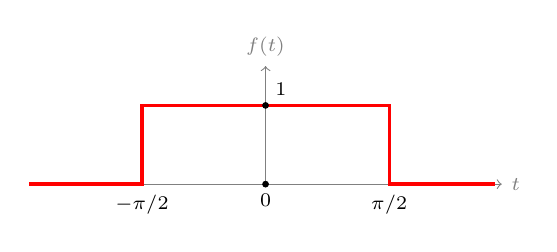
\begin{tikzpicture}
      \draw[->,gray] (-3,0) -- (3,0) node[right] {\scriptsize$t$};
      \draw[->,gray] (0,0) -- (0,1.5) node[above] {\scriptsize$f(t)$};
      \draw[very thick,red] (-3,0) -- (-1.57,0) node[below, black] {\scriptsize$-\pi/2$} -- (-1.57,1) -- (1.57,1) 
      -- (1.57,0) node[below, black] {\scriptsize$\pi/2$} -- (2.92,0);
      \draw[fill] (0,1) circle (1pt) node[above right] {\scriptsize$1$};
      \draw[fill] (0,0) circle (1pt) node[below] {\scriptsize$0$};
    \end{tikzpicture}
    \caption{Función cajón o pulso rectangular.}
    \label{fig:pulso_rectangular}
  \end{figure}
  Para conocer el espectro de frecuencias necesitamos calcular la transformada de Fourier del pulso rectangular. Entonces, aplicando la definición de transformada (ecuación \eqref{eq:transformada_definicion_formal}), necesitamos calcular
  $$
  F(\omega) = \int_{-\infty}^\infty f(t)e^{-j\omega t}dt
  $$
  Observando la función $f(t)$, resulta claro que la integral se puede desdoblar en tres integrales. Como la función la podemos definir por partes como:
  $$
  f(t)=\begin{cases}
    0 & t < -\pi/2 \\ 
    1 & -\pi/2\leq t \leq \pi/2 \\ 
    0 & \pi/2 < t
  \end{cases}
  $$
  Entonces la integral sobre el intervalo $(-\infty,\infty)$ es 
  $$
  \int_{-\infty}^\infty f(t)e^{-j\omega t}dt = \int_{-\infty}^{-\pi/2} f(t)e^{-j\omega t}dt + \int_{-\pi/2}^{\pi/2} f(t)e^{-j\omega t}dt + \int_{\pi/2}^\infty f(t)e^{-j\omega t}dt
  $$
  Donde, la integral en el intervalo $(-\infty,-\pi/2)$ y $(\pi/2,\infty)$ son cero. Entonces, resulta 
  $$
    F(\omega) = \int_{-\pi/2}^{\pi/2} (1)e^{-j\omega t}dt = \left.-\frac{e^{-j\omega t}}{j\omega} \right\rvert_{-\pi/2}^{\pi/2}
  $$
  Operando algebraicamente,
  \begin{align*}
              &= \frac{1}{j\omega}(e^{j\omega(\pi/2)}-e^{-j\omega(\pi/2)}) \\ 
              &= \frac{2}{2}\cdot \frac{1}{j\omega}(e^{j\omega(\pi/2)}-e^{-j\omega(\pi/2)}) \\ 
    F(\omega) &= \frac{2}{\omega}\sin\left(\frac{\omega\pi}{2}\right)  
  \end{align*}
  Y de esta última expresión puede obtenerse una función muy elegante, llamada \textit{seno cardinal}, que se define como $\sin(x)/x$. Para obtener esta expresión multiplicamos y dividimos entre $\pi$, 
  $$
  \pi\frac{2}{\pi\omega}\sin\left(\frac{\omega\pi}{2}\right) = \pi \left[\frac{1}{(\pi\omega)/2}\sin\left(\frac{\omega\pi}{2}\right)\right]
  $$
  resultando 
  $$
  \boxed{F(\omega) = \pi\sinc\left(\frac{\omega\pi}{2}\right)}
  $$
  \begin{figure}[ht]
    \centering
    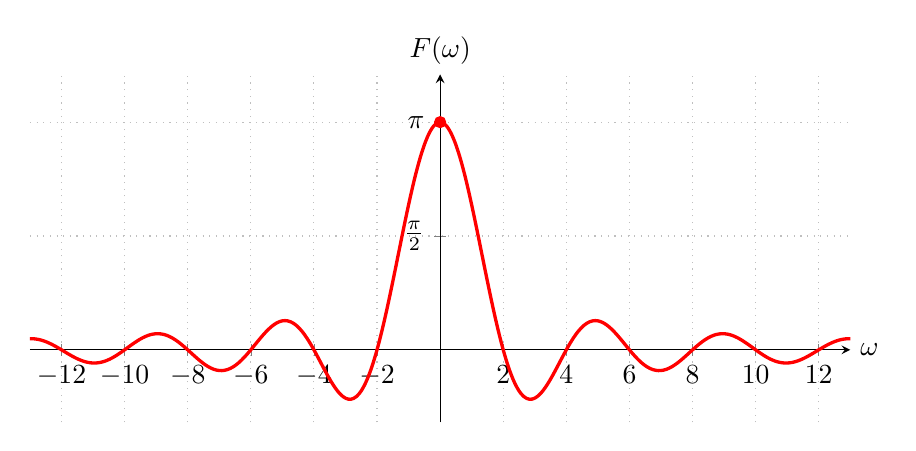
\begin{tikzpicture}
      \begin{axis}[
        axis lines = middle,
        xlabel = $\omega$,
        ylabel = $F(\omega)$,
        ymin = -1, ymax = 3.8,
        xmin = -13, xmax = 13,
        grid = major,
        grid style = dotted,
        width = 12cm, height = 6cm,
        % Estilo de las etiquetas
        every axis x label/.style={at={(current axis.right of origin)},anchor=west},
        every axis y label/.style={at={(current axis.above origin)},anchor=south},
        ytick = {-1.5708, 0, 1.5708, 3.14159}, 
        yticklabels = {$-\frac{\pi}{2}$, $0$, $\frac{\pi}{2}$, $\pi$},
        xtick = {-12,-10,-8,-6,-4,-2,2,4,6,8,10,12}
      ]
        
        \addplot [
            domain=-13:13, 
            samples=300,
            color=red, 
            very thick,
            smooth
        ] 
        % Si x es 0, devuelve 1. Si no, calcula sin(x en grados)/x
        {x == 0 ? pi : pi * sin(deg(x*pi/2))/(x*pi/2)};
        \addplot[mark=*, color=red] coordinates {(0,3.14159)};
      \end{axis}
    \end{tikzpicture}
    \caption{Gráfico de $F(\omega)$ de la función cajón.}
  \end{figure}
  El espectro continuo (o función de la frecuencia continua), dado por la curva envolvente de la función seno cardinal, es llamado \textit{espectro de banda}. Mientras que el espectro discreto, si se toman solo las ordenadas para cada valor de la frecuencia $[\omega=k\omega_0]$, es el \textit{espectro de línea}. Gráficamente se vería algo como lo representado en la figura \ref{fig:espectro_discreto_para_cajon}.
  \begin{figure}[ht]
    \centering
    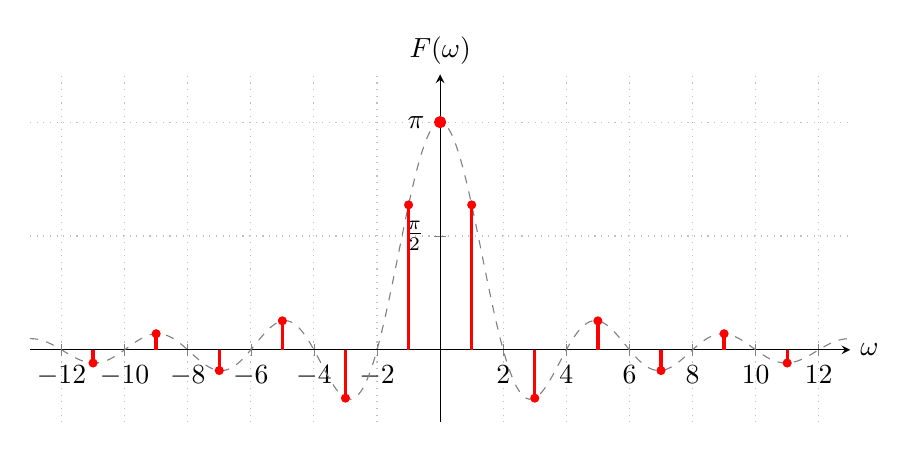
\begin{tikzpicture}
      \begin{axis}[
        axis lines = middle,
        xlabel = $\omega$,
        ylabel = $F(\omega)$,
        ymin = -1, ymax = 3.8,
        xmin = -13, xmax = 13,
        grid = major,
        grid style = dotted,
        width = 12cm, height = 6cm,
        % Estilo de las etiquetas
        every axis x label/.style={at={(current axis.right of origin)},anchor=west},
        every axis y label/.style={at={(current axis.above origin)},anchor=south},
        ytick = {-1.5708, 0, 1.5708, 3.14159}, 
        yticklabels = {$-\frac{\pi}{2}$, $0$, $\frac{\pi}{2}$, $\pi$},
        xtick = {-12,-10,-8,-6,-4,-2,2,4,6,8,10,12}
      ]
        
        \addplot [
            domain=-13:13, 
            samples=300,
            color=gray, 
            thin,
            dashed,
            smooth
        ] 
        % Si x es 0, devuelve 1. Si no, calcula sin(x en grados)/x
        {x == 0 ? pi : pi * sin(deg(x*pi/2))/(x*pi/2)};

        \addplot [
            ycomb,              % Tipo de gráfico "peine"
            color=red,
            very thick,
            mark=*,             % Pone un punto al final de la línea (opcional)
            mark options={scale=0.5},
            % Aquí definimos exactamente dónde quieres las líneas:
            samples at={-11,-9,...,-1, 1,3,...,11} 
        ] 
        % Reutilizamos la MISMA fórmula matemática
        {x == 0 ? pi : pi * sin(deg(x*pi/2))/(x*pi/2)};

        \addplot[mark=*, color=red] coordinates {(0,3.14159)};
      \end{axis}
    \end{tikzpicture}
    \caption{Gráfico de espectro discreto para $F(\omega)$.}
    \label{fig:espectro_discreto_para_cajon}
  \end{figure}

  Si quisiera expresarse la función del tiempo que corresponde al pulso rectangular, podría encontrarse a partir de la integral:
  $$
  f(t)=\frac{1}{2}\int_{-\pi/2}^{\pi/2} \sinc\left(\frac{\omega\pi}{2}\right)e^{j\omega t}d\omega
  $$
  que es la función del tiempo que describe analíticamente al pulso rectangular.
\end{example}

Ahora, consideremos la transformada de algunas funciones simples, tales como la función constante, el coseno y la exponencial.

\begin{example}[Función constante]
  Sea la función constante unitaria: 
  $$
  f(t)=1
  $$
  \begin{figure}[ht]
    \centering
    \begin{subfigure}[b]{.48\textwidth}
      \centering
      \begin{tikzpicture}
        \draw[->,gray] (-3,0) -- (3,0) node[right] {\scriptsize$t$};
        \draw[->,gray] (0,-.2) -- (0,1.3) node[above] {\scriptsize$f(t)$};
        \draw[very thick,red] (-3,1) -- (3,1) node[midway,below right,black] {\scriptsize$1$};
        \node[below right] at (0,0) {\scriptsize$0$}; 
        \draw[fill] (0,1) circle (1pt);
      \end{tikzpicture}
      \caption{Gráfico de la función unitaria.}
    \end{subfigure}
    \hfill
    \begin{subfigure}[b]{.48\textwidth}
      \centering
      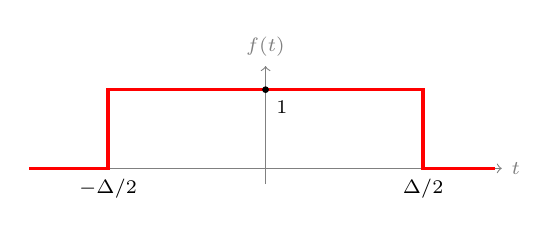
\begin{tikzpicture}
        \draw[->,gray] (-3,0) -- (3,0) node[right] {\scriptsize$t$};
        \draw[->,gray] (0,-.2) -- (0,1.3) node[above] {\scriptsize$f(t)$};
        \draw[very thick,red] (-3,0) -- (-2,0) node[below,black] {\scriptsize$-\Delta/2$} -- (-2,1) -- 
          (2,1) node[midway,below right,black] {\scriptsize$1$} -- (2,0) node[below,black] {\scriptsize$\Delta/2$} -- (2.92,0);
        \draw[fill] (0,1) circle (1pt);
      \end{tikzpicture}
      \caption{Gráfico del pulso en $[-\Delta/2,\Delta/2]$.}
    \end{subfigure}
    \caption{}
    \label{fig:ej:constante_unitaria}
  \end{figure}
  Suponiendo que, en el caso del ejemplo del pulso rectangular anterior, éste hubiera tenido duración $\Delta$, se podría interpretar al la función constante unitaria como un pulso de duración $\Delta\to\infty$, como muestra la figura \ref{fig:ej:constante_unitaria}.

  Entonces, la transformada podría resolverse usando el resultado del ejemplo anterior, haciendo:
  $$
  F(\omega) = \lim_{\Delta \to \infty}\left(\Delta \sinc\left(\frac{\omega\Delta}{2}\right)\right)
  $$
  Y, multiplicando por $2\pi$, resulta:
  $$
  F(\omega) = 2\pi \lim_{ \Delta\to \infty}\left(\frac{\Delta}{2\pi} \sinc\left(\frac{\omega\Delta}{2}\right)\right)
  $$
  Donde puede demostrarse que ese límite equivale a un impulso al origen de la variable $\omega$. Intuitivamente, se aprecia que la función seno cardinal tiende a cero para $\Delta \to\infty$, pero permanece un factor $\Delta$ en el numerador que lleva el resultado a ser un impulso:
  $$
  F(\omega) = 2\pi\delta(\omega)
  $$
  donde $\delta(\omega)$ es la función delta de Dirac. Esta es la transformada de Fourier de la función constante unitaria expresada por un impulso unitario de energía $2\pi$.
  \begin{figure}[ht]
    \centering
    \begin{tikzpicture}
      \draw[->,gray] (-2,0) -- (2,0) node[right] {\scriptsize$\omega$};
      \draw[->,gray] (0,-.2) -- (0,1.3) node[above] {\scriptsize$F(\omega)$};
      \draw[very thick,red,->] (0,0) -- (0,1) node[below right,black] {\scriptsize$2\pi\delta(\omega)$};
    \end{tikzpicture}
    \caption{Gráfico de la transformada $\mathcal{F}\{f(t)=1\}$.}
  \end{figure}
\end{example}
